%%%%%%%%%%%%%%%%%%%%%%%%%%%%%%%%%%%%%%%%%%%%%%%%
%%   TEMPLATE MAIN FILE                       %%
%%%%%%%%%%%%%%%%%%%%%%%%%%%%%%%%%%%%%%%%%%%%%%%%

\documentclass[10pt,reqno,sumlimits]{amsart}
\usepackage{amssymb}
\usepackage{epsfig}
\usepackage{multirow}
\usepackage{graphics}
\usepackage{graphicx}
\usepackage{subfigure}
\usepackage{url}
%\textwidth 6.2in
%\oddsidemargin.20in
%\evensidemargin.35in
%%\lineskip 1in
%%\baselineskip.55cm

% Read in specially defined commands
% Change margins and baselinestretch in draft mode
\def\draft{
% make margins smaller
\addtolength{\oddsidemargin}{-0.5in}
\addtolength{\topmargin}{-0.65in}
\addtolength{\textheight}{1in}
\addtolength{\textwidth}{1.5in}
% A more reasonable baselinestretch, is still nearly doublespaced.
\def\baselinestretch{1.4}
}

%\vfuzz2pt % Don't report over-full v-boxes if over-edge is small
%\hfuzz2pt % Don't report over-full h-boxes if over-edge is small

%%%%%%%%%%%%%%%%%%%%%%%%%%%%%%%%%%%%%%%%%%%%%%%%%%%%%%%%
%%              Theorems                               %
%%%%%%%%%%%%%%%%%%%%%%%%%%%%%%%%%%%%%%%%%%%%%%%%%%%%%%%%
\theoremstyle{plain}
\newtheorem{theorem}{Theorem}
\newtheorem{corollary}[theorem]{Corollary}
\newtheorem{lemma}[theorem]{Lemma}
\newtheorem{proposition}[theorem]{Proposition}
\newtheorem{conjecture}[theorem]{Conjecture}

\theoremstyle{definition}
\newtheorem{remark}[theorem]{Remark}
\newtheorem{definition}[theorem]{Definition}
\newtheorem{example}[theorem]{Example}
\newtheorem{notation}{Notation}

%%%%%%%%%%%%%%%%%%%%%%%%%%%%%%%%%%%%%%%%%%%%%%%%%%%%%%%%
%%      Definitions and Commands                       %
%%%%%%%%%%%%%%%%%%%%%%%%%%%%%%%%%%%%%%%%%%%%%%%%%%%%%%%%
\newcommand{\A}{{\mathbb A}}
\newcommand{\R}{{\mathbb R}}
\newcommand{\Q}{{\mathbb Q}}
\newcommand{\C}{{\mathbb C}}
\newcommand{\D}{{\mathbb D}}
\newcommand{\Z}{{\mathbb Z}}
\newcommand{\h}{{\mathbb H}}
\newcommand{\CP}{{\mathbb C}{\mathbb P}}
\newcommand{\I}{{\mathbb I}}
\newcommand{\N}{{\mathbb N}}
%
\newcommand{\calA}{{\mathcal A}}
\newcommand{\calB}{{\mathcal B}}
\newcommand{\calC}{{\mathcal C}}
\newcommand{\calD}{{\mathcal D}}
\newcommand{\calE}{{\mathcal E}}
\newcommand{\calF}{{\mathcal F}}
\newcommand{\calG}{{\mathcal G}}
\newcommand{\calH}{{\mathcal H}}
\newcommand{\calI}{{\mathcal I}}
\newcommand{\calK}{{\mathcal K}}
\newcommand{\calM}{{\mathcal M}}
\newcommand{\calO}{{\mathcal O}}
\newcommand{\calP}{{\mathcal P}}
\newcommand{\calR}{{\mathcal R}}
\newcommand{\calS}{{\mathcal S}}
\newcommand{\calL}{{\mathcal L}}
\newcommand{\calX}{{\mathcal X}}
\newcommand{\calU}{{\mathcal U}}
\newcommand{\calV}{{\mathcal V}}
\newcommand{\calZ}{{\mathcal Z}}
%
\newcommand{\ggoth}{{\mathfrak  g}}
\newcommand{\ugoth}{{\mathfrak  u}}
\newcommand{\hgoth}{{\mathfrak  h}}
%%
\newcommand{\1}{{\bf 1}}
\newcommand{\acts}{{\circlearrowright}}
\newcommand{\ex}[1]{{e^{#1}}}
\newcommand{\dd}[2]{\frac{\partial #1}{\partial #2}}
\newcommand{\iso}{\stackrel{\simeq}{\longrightarrow}}
\newcommand{\spinc}{$\text{spin}^c$}
\newcommand{\Dirac}{\not\!\!D}
\newcommand{\inc}{\hookrightarrow}
%%
\newcommand{\Aut}{\operatorname{Aut}}
\newcommand{\Hom}{\operatorname{Hom}}
\newcommand{\Hor}{\operatorname{Hor}}
\newcommand{\Ext}{\operatorname{Ext}}
\newcommand{\End}{\operatorname{End}}
\newcommand{\Map}{\operatorname{Map}}
\newcommand{\Diff}{\operatorname{Diff}}
\newcommand{\Tr}{\operatorname{Tr}}
\newcommand{\Lie}{\operatorname{Lie}}
\newcommand{\ad}{{\operatorname{ad\,}}}
\newcommand{\sign}{{\operatorname{sign}}}
\newcommand{\grad}{{\operatorname{grad}}}
\newcommand{\coker}{{\operatorname{coker}}}
\newcommand{\dett}{{\operatorname{det}}}
\newcommand{\ch}{{\operatorname{ch}}}
\newcommand{\rk}{{\operatorname{rk}}}
\newcommand{\maxx}{{\operatorname{max}}}
\newcommand{\minn}{{\operatorname{min}}}
\newcommand{\id}{{\operatorname{id}}}
\newcommand{\ind}{{\operatorname{ind}}}
\newcommand{\Ind}{{\operatorname{Ind}}}
\newcommand{\spann}{{\operatorname{span}}}
\newcommand{\Spin}{{\operatorname{Spin}}}
\newcommand{\Pin}{{\operatorname{Pin}}}
\newcommand{\im}{{\operatorname{Im}}}
\renewcommand{\Im}{{\operatorname{Im}}}
\newcommand{\dimm}{{\operatorname{dim}}}
\newcommand{\cl}{{\operatorname{cl}}}
%%
\newcommand{\tM}{{\tilde{M}}}
\newcommand{\tC}{{\tilde{C}}}
\newcommand{\tE}{{\tilde{E}}}
\newcommand{\tF}{{\tilde{F}}}
\newcommand{\talpha}{{\tilde{\alpha}}}
%%
\newcommand{\zbar}{\overline{z}}
\newcommand{\wbar}{\overline{w}}
\newcommand{\phibar}{\overline{\phi}}
\newcommand{\psibar}{\overline{\psi}}
\newcommand{\Bbar}{\overline{B}}
\newcommand{\Cbar}{\overline{C}}
\newcommand{\inv}{^{-1}}
%%      
\newcommand{\rb}[1]{\raisebox{0pt}[0pt][0pt]{#1}}
\newsavebox{\savepar}
\newenvironment{boxit}{\begin{lrbox}{\savepar}\begin{minipage}[b]{.5in}}
{\end{minipage}\end{lrbox}\fbox{\usebox{\savepar}}}
%%\newcommand{\ip}[1]{\langle\! #1 \! \rangle}
\newcommand{\ip}[1]{\langle #1 \rangle}
\newcommand{\norm}[1]{\| #1 \|}
%
%\newcommand{\remark}{{\tt ?}\marginpar{\Large\centering ?}}
\newcommand{\rremark}{\marginpar{\Large\centering ?}}
\newcommand{\Remark}[1]{\textsc{\tiny{[#1]}}\rremark}
\newcommand{\todo}{\textsc{Todo!}\marginpar{\Large\centering !}}
%
\numberwithin{equation}{section}
\renewcommand{\theequation}{{\thesection{.}}\arabic{equation}}
\newcounter{dummy}
%
%%%%%%%%%%%%%%%%%%%%%%%%%%%%%%%%%%%%%%%%%%%%%%%%%%%%%%%
\begin{document}

\title[Assignment 2]{Grammatically Correct}
\author{Joe Smith}


%\begin{abstract}
%The abstract
%\end{abstract}

\maketitle

%\tableofcontents

%%%%%%%%%%%%%%%%%%%%%%%%%%%%%%%%%%%%%%%%%%%%%%%%%%%%%%%

\section {Parse Trees}
\begin{figure}[htbp]
\centerline{
    \mbox{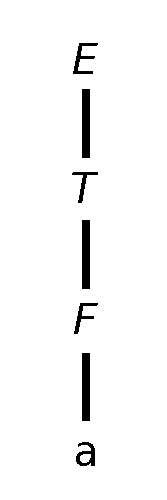
\includegraphics[height=1.5in]{3_1_a.pdf}}
  }
  \caption{$a$}
  \label{fig:fit}
\end{figure}

\begin{figure}[htbp]
\centerline{
    \mbox{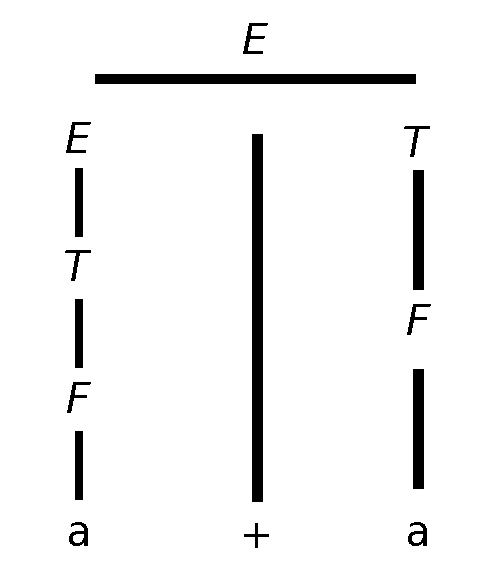
\includegraphics[width=1.5in]{3_1_b.pdf}}
  }
  \caption{$a + a$}
  \label{fig:fit}
\end{figure}

\begin{figure}[htbp]
\centerline{
    \mbox{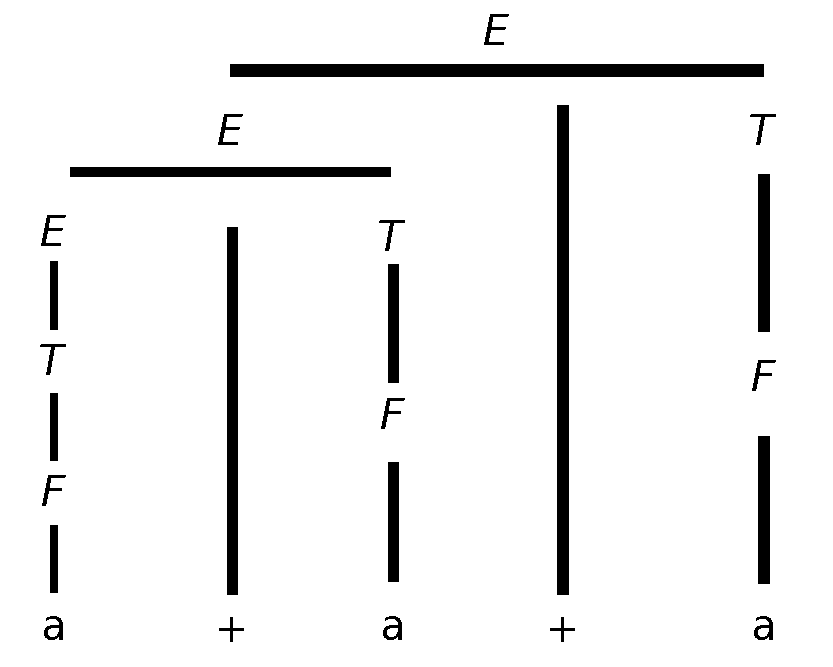
\includegraphics[width=1.5in]{3_1_c.pdf}}
  }
  \caption{$a + a + a$}
  \label{fig:fit}
\end{figure}

\begin{figure}[htbp]
\centerline{
    \mbox{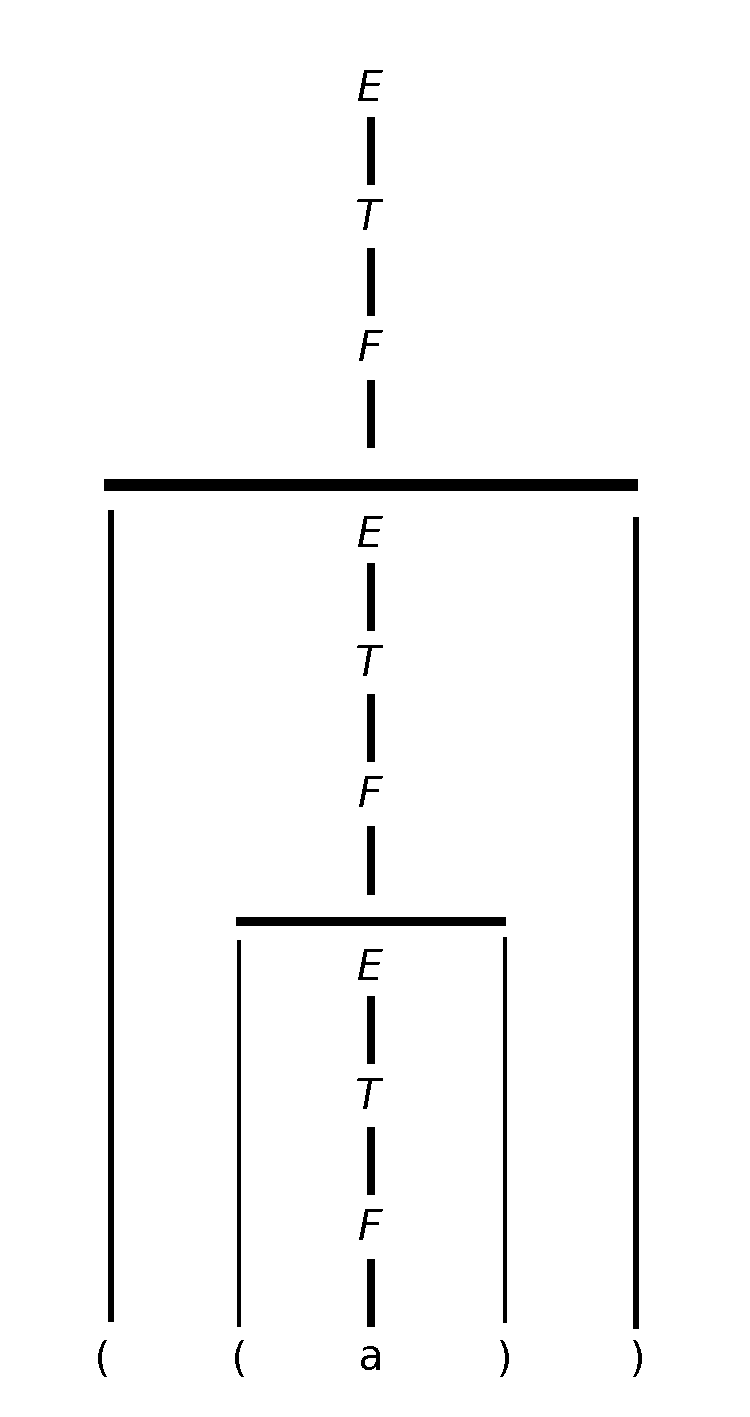
\includegraphics[width=1.5in]{3_1_d.pdf}}
  }
  \caption{$((a))$}
  \label{fig:fit}
\end{figure}

\section {Creating Fine Greatness (CFG)}
\begin{enumerate}
\item \{$w|w$ contains at least three 1s\}

\hspace{0.3in}$S\rightarrow\ T\ T\ T$

\hspace{0.3in}$T\rightarrow\ U1U$

\hspace{0.3in}$U\rightarrow\ \Sigma\ |\ U\Sigma\ |\ \Sigma U$

\item \{$w|w$ starts and ends with the same symbol\}

\hspace{0.3in}$S\rightarrow\ 0T0 | 1T1$

\hspace{0.3in}$T\rightarrow\ \Sigma T | T\Sigma | \Sigma$

\hspace{0.3in}
\item \{$w|w$ contains more 1s than 0s\}

\hspace{0.3in}

\end{enumerate}

\section {Public Display of Aff--... Push Down Automata}

\begin{figure}[htbp]
\centerline{
    \mbox{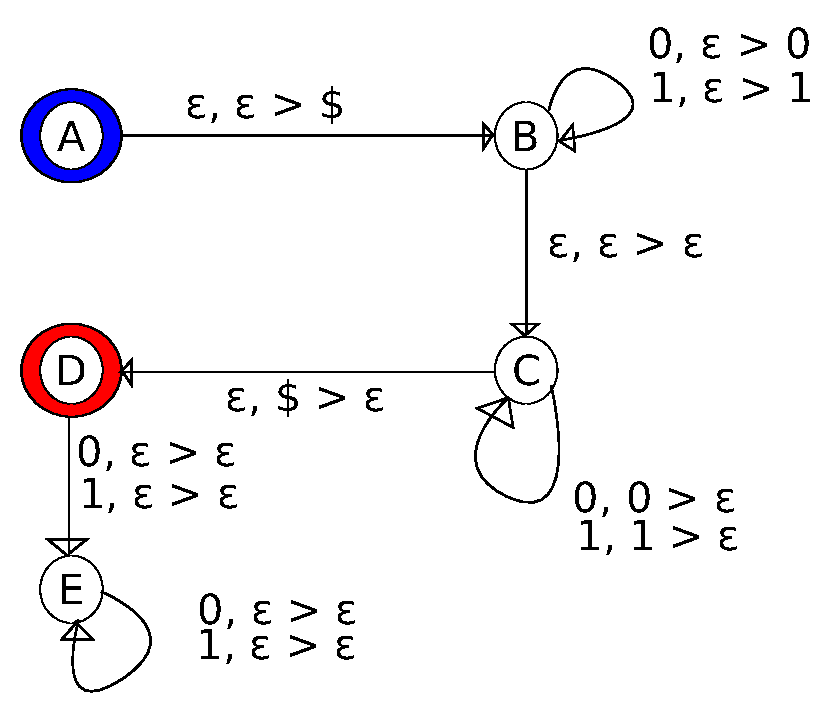
\includegraphics[width=2in]{3_3.pdf}}
  }
  \caption{$\{ww^r |w \in \{0, 1\}^∗ \}$}
  \label{fig:fit}
\end{figure}

\section {CFLs closed under Union}

\section {I spent all night Pumping}

\end{document}

%%%%%%%%%%%%%%%%%%%%%%%%%%%%%%%%%%%%%%%%%%%%%%%%%%%%%%%

%%% Local Variables: 
%%% mode: latex
%%% TeX-master: "main"
%%% End: 

